\documentclass[a4paper]{article}
\usepackage[spanish]{babel}
\usepackage[utf8]{inputenc}
\usepackage{charter}   % tipografia
\usepackage{graphicx}
%\usepackage{makeidx}
\usepackage{paralist} %itemize inline
\usepackage{float}
\restylefloat{table}

%\usepackage{float}
%\usepackage{amsmath, amsthm, amssymb}
%\usepackage{amsfonts}
%\usepackage{sectsty}
%\usepackage{charter}
%\usepackage{wrapfig}
%\usepackage{listings}
%\lstset{language=C}


\usepackage{color} % para snipets de codigo coloreados
\usepackage{fancybox}  % para el sbox de los snipets de codigo

\definecolor{litegrey}{gray}{0.94}

% \newenvironment{sidebar}{%
% 	\begin{Sbox}\begin{minipage}{.85\textwidth}}%
% 	{\end{minipage}\end{Sbox}%
% 		\begin{center}\setlength{\fboxsep}{6pt}%
% 		\shadowbox{\TheSbox}\end{center}}
% \newenvironment{warning}{%
% 	\begin{Sbox}\begin{minipage}{.85\textwidth}\sffamily\lite\small\RaggedRight}%
% 	{\end{minipage}\end{Sbox}%
% 		\begin{center}\setlength{\fboxsep}{6pt}%
% 		\colorbox{litegrey}{\TheSbox}\end{center}}

\newenvironment{codesnippet}{%
	\begin{Sbox}\begin{minipage}{\textwidth}\sffamily\small}%
	{\end{minipage}\end{Sbox}%
		\begin{center}%
		\vspace{-0.4cm}\colorbox{litegrey}{\TheSbox}\end{center}\vspace{0.3cm}}



\usepackage{fancyhdr}
\pagestyle{fancy}

%\renewcommand{\chaptermark}[1]{\markboth{#1}{}}
\renewcommand{\sectionmark}[1]{\markright{\thesection\ - #1}}

\fancyhf{}

\fancyhead[LO]{Sección \rightmark} % \thesection\ 
\fancyfoot[LO]{\small{Aldasoro, Chamo, Galli, Noriega, Previgliano \& Zimenspitz}}
\fancyfoot[RO]{\thepage}
\renewcommand{\headrulewidth}{0.5pt}
\renewcommand{\footrulewidth}{0.5pt}
\setlength{\hoffset}{-0.8in}
\setlength{\textwidth}{16cm}
%\setlength{\hoffset}{-1.1cm}
%\setlength{\textwidth}{16cm}
\setlength{\headsep}{0.5cm}
\setlength{\textheight}{25cm}
\setlength{\voffset}{-0.7in}
\setlength{\headwidth}{\textwidth}
\setlength{\headheight}{13.1pt}

\renewcommand{\baselinestretch}{1.1}  % line spacing


% \setcounter{secnumdepth}{2}
\usepackage{underscore}
\usepackage{caratula}
\usepackage{url}


% ******************************************************** %
%              TEMPLATE DE INFORME ORGA2 v0.1              %
% ******************************************************** %
% ******************************************************** %
%                                                          %
% ALGUNOS PAQUETES REQUERIDOS (EN UBUNTU):                 %
% ========================================
%                                                          %
% texlive-latex-base                                       %
% texlive-latex-recommended                                %
% texlive-fonts-recommended                                %
% texlive-latex-extra?                                     %
% texlive-lang-spanish (en ubuntu 13.10)                   %
% ******************************************************** %



\begin{document}


\thispagestyle{empty}
\materia{Ingenier\'ia de Software I}
\submateria{Segundo Cuatrimestre de 2015}
\titulo{Trabajo Práctico I}
\subtitulo{An\'alisis preliminar del Sistema Electoral Nacional de Voto Electr\'onico \textbf{(SVE)}}
\integrante{Aldasoro Agustina}{86/13}{agusaldasoro@gmail.com}
\integrante{Chamo Nicolás}{282/13}{nicochamo@hotmail.com}
\integrante{Galli Cristian}{538/11}{lococris88@hotmail.com}
\integrante{Noriega Francisco}{660/12}{frannoriega.92@gmail.com}
\integrante{Previgliano Fabricio}{430/13}{fjprevi@gmail.com}
\integrante{Zimenspitz Ezequiel}{155/13}{ezeqzim@gmail.com}

\maketitle
\newpage

\thispagestyle{empty}
\vfill
\thispagestyle{empty}
\vspace{3cm}
\tableofcontents
\newpage

\section{Descripci\'on de la m\'aquina a utilizar}

El sistema que proponemos, puede subdividirse en dos estad\'ios: uno que es el que se relaciona al centro de c\'omputos; y otro que se corresponde con la emisi\'on de los votos.\\

El primero es un software utilizable en PC's tradicionales, que admite carga del padr\'on; designaci\'on de presidentes de mesa; distribuci\'on de presidentes de mesa y electores en las distintas escuelas y mesas del pa\'is; cargar los candidatos de cada partido pol\'itico; proveer constrase\~nas para los fiscales generales de cada escuela; recibir los resultados de las elecciones de cada escuela y publicar toda la informaci\'on necesaria en una p\'agina web.\\

El segundo consta de una m\'aquina especialmente dise\~nada para actos de sufragio. Cada m\'aquina impresora de voto posee una pantalla t\'actil en la que se muestran las distintas opciones posibles a votar seg\'un el modo en el que este iniciada; una ranura para insertar una boleta; una impresora que grabar\'a la decisi\'on del elector en la boleta y en el chip de la misma; un lector de c\'odigos de boleta para la etapa del recuento de votos y para que el elector verifique la correctitud de su voto; una entrada para auriculares; un espacio para bater\'ia externa con su bater\'ia cargada y colocada (la cual posee una duraci\'on de tres horas); una entrada para conexi\'on telef\'onica a internet. En la etapa de conteo, la m\'aquina lleva cuenta de los votos que se vayan verificando y no sean impugnados

\newpage
\section{Diagrama de Objetivos}

\subsection{Criterios preliminares}

A la hora de encarar un problema como el siguiente es importante identificar subproblemas que 
nos permitan construir de manera más simple una solución al mismo. En este caso identificamos que 
el problema de una elección puede dividirse temporalmente en tres etapas claras:

\begin{enumerate}
\item El proceso de preparación anterior al día de las elecciones.
\item El día de las elecciones.
\item El conteo de los votos emitidos.
\end{enumerate}

Se puede entonces decir que para lograr una elección exitosa necesitamos que estas tres etapas lo sean.\\

Este criterio será la base para la construcción del Diagrama de objetivos que modela los requerimientos necesarios del software.	\\

A continuación presentaremos el diagrama de objetivos del problema acompañado de un conjunto de escenarios descriptos de manera informal que ayudan a comprender el mismo.\\

A su vez consideramos la siguientes hipótesis de dominio:

\begin{itemize}
\item Todas las escuelas tienen conexión telefónica.
\item \textcolor{red}{Ponemos algo de las computadoras en red para el o-refinamiento?}
\end{itemize}

\newpage
\subsection{Diagrama}

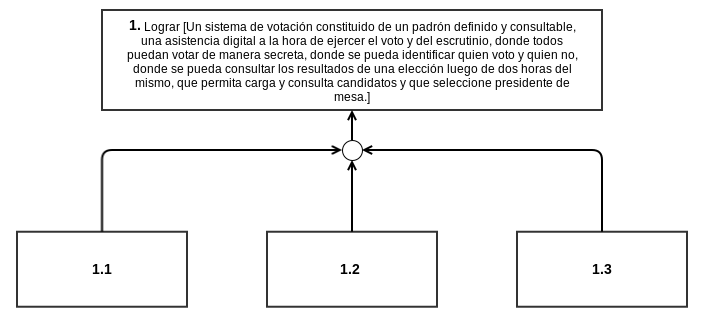
\includegraphics[scale=0.55]{imagenes/Diagramas/1.png}
\newpage
\section{Diagrama de Objetivos (1.1)}

\subsection{Descripci\'on: Preparación}

En la etapa de preparación, el Ministerio provee un listado con los datos personales de todo el padrón, y lo carga en el sistema, junto con el código fuente del mismo, permitiendo así la exposición de los datos a través de la interfaz web. De esta manera, un elector podrá consultar el padrón, y de no figurar en él, se dirigirá al ministerio, donde el sistema le permitirá al ministerio ingresar nuevos votantes  (hasta determinada fecha límite) asignándoles una mesa válida. A su vez, electores, fiscales generales y partidos políticos, podrán revisar el código y ver que no haya ninguna irregularidad en el mismo.

Pasada dicha fecha, el ministerio suministra la información sobre las escuelas disponibles para votar al sistema, y procede a activar la opción “Asignar escuela y mesa” a cada elector, donde el sistema realiza dicha asignación automáticamente. A su vez, asigna de manera aleatoria los presidentes de mesas, ponderando a los que nunca lo fueron previamente.\\

Dado que el ministerio precisa conocer a los presidentes de mesa designados, el sistema permite consultar quienes son los mismos, de manera que el Ministerio pueda comunicarse con ellos. En caso de que algún notificado no pudiera estar presente (con justificación válida), el sistema permitirá al Ministerio elegir uno nuevo. Quedará a cargo del Ministerio, la capacitación de los mismos.\\

Posteriormente, los partidos políticos presentan sus candidatos al Ministerio (hasta determinada fecha límite). Pasada la misma, el Ministerio carga esta información en la versión Web para que esté disponible a consultar y el equipo técnico del mismo graba la información en las máquinas impresoras de voto. En este momento, también, asigna una máquina impresora de voto a cada mesa, más dos extra por escuela (en caso de que suceda algún exabrupto), sumado a una máquina extra (que sólo será utilizada para el envío de datos de resultados) y un cable de conexión de teléfono. Cada máquina posee una batería que dura 3 hs sin estar conectada a alimentación eléctrica. El sistema proveerá una contraseña única para todas las máquinas para entrar en el “Modo envío” y ademas una contraseña única por Fiscal General de escuela, los cuales se utilizarán en el momento de cargar los resultados de la elección.\\

Luego, se prepara un lote de boletas para cada mesa, considerando entre ellas a la boleta donde se imprimirán los resultados. Por cada mesa, se asignan además una cantidad extra de boletas, en caso de que algún votante termine utilizando más de una (dado que se puede arrepentir antes de efectuar su voto). Las boletas tienen dos troqueles iguales, los cuales permiten identificar que la misma no fue intercambiada por el votante al momento de realizar la elección, evitando así este tipo de fraude. Las mismas tienen un espacio para impresión con tinta, y un chip grabable dentro.\\

Después, el Ministerio imprime copias del padrón correspondiente a cada mesa, para que sean utilizados por los presidentes de mesa, fiscales y las escuelas, estas mismas lo deberán dejar en un lugar visible para que los votantes puedan consultarlo. También prepara las urnas, armando tantas como cantidad de mesas haya, las cuales poseen una identificación de la mesa a la que pertenecen; y provee un par de auriculares para cada escuela, que recibirán los encargados de las mismas, los cuales brindarán a los votantes no videntes una ayuda a la hora del sufragio. Es el ministerio también el encargado de entregarle a cada Fiscal General las dos contraseñas, \textcolor{red}{y un pendrive que se insertará en las máquinas, para veríficar que el checksum sea correcto.}

Una vez está todo preparado, el Ministerio notifica a las fuerzas de seguridad las escuelas seleccionadas para la elección donde deberán brindar aporte.\\

Llegado el dia de la elección, el correo lleva a cada escuela correspondiente, la cantidad de máquinas de voto asignadas junto a las máquinas extra, todas con sus baterías correspondientes. Además, lleva las boletas, las urnas, las copias del padrón y los auriculares. Todo esto es recibido por el encargado, quien se los otorgará a los presidente de mesa y fiscales. Una vez allí, el fiscal general junto a los presidentes de mesa que ya estén presentes y las fuerzas de seguridad, distribuyen una mesa por aula. A su vez, se posicionan las urnas, las boletas y las máquinas de votación en su lugar correspondiente. El par de auriculares permanecerá en posesión del Fiscal General, quien será el encargado de otorgarlo de ser necesario.

Cada presidente de mesa se ubica en su mesa respectiva. Si llega un votante a una mesa, y esta no cuenta con un presidente de mesa, el fiscal general de la escuela lo nombrará como presidente de dicha mesa. Cada presidente de mesa da inicio a la votación. Lo hace al activar una opción en la máquina de votación. El presidente de mesa es quien emitirá su voto primero acorde a lo explicado posteriormente. A partir de ese momento, cualquier votante habilitado que llegue a su mesa podrá emitir sufragio.

\newpage
\subsection{Diagrama}

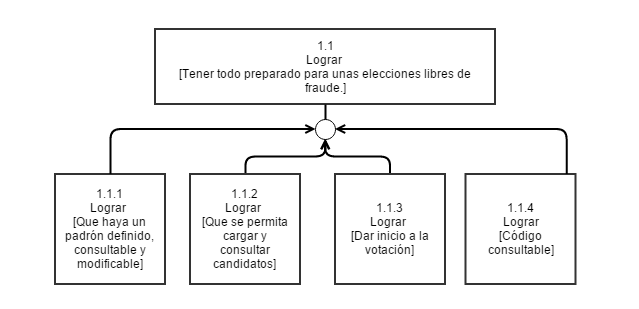
\includegraphics[scale=0.55]{imagenes/Diagramas/11/11.png}
\\
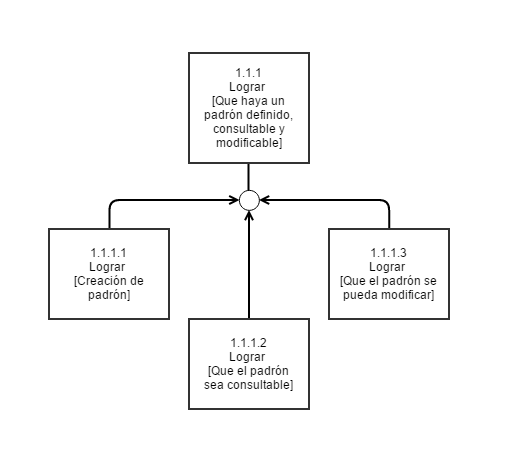
\includegraphics[scale=0.55]{imagenes/Diagramas/11/111.png}
\\
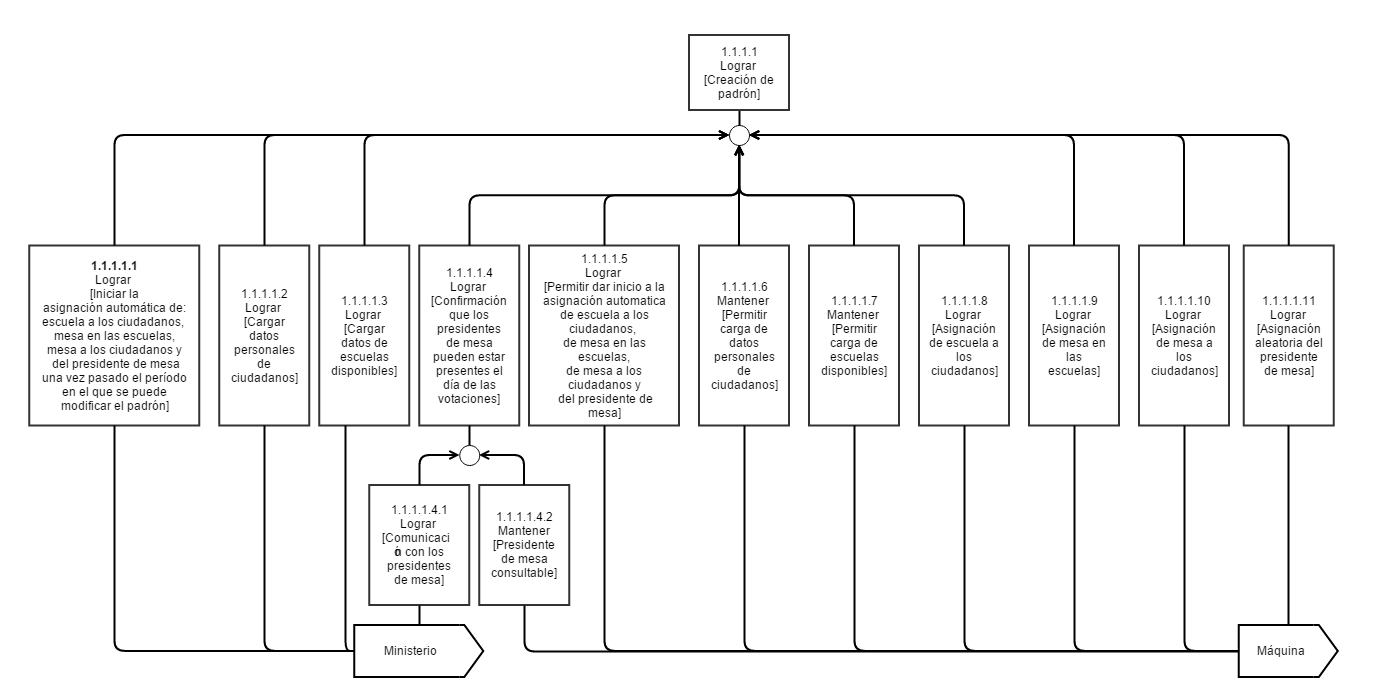
\includegraphics[scale=0.45]{imagenes/Diagramas/11/1111.png}
\\
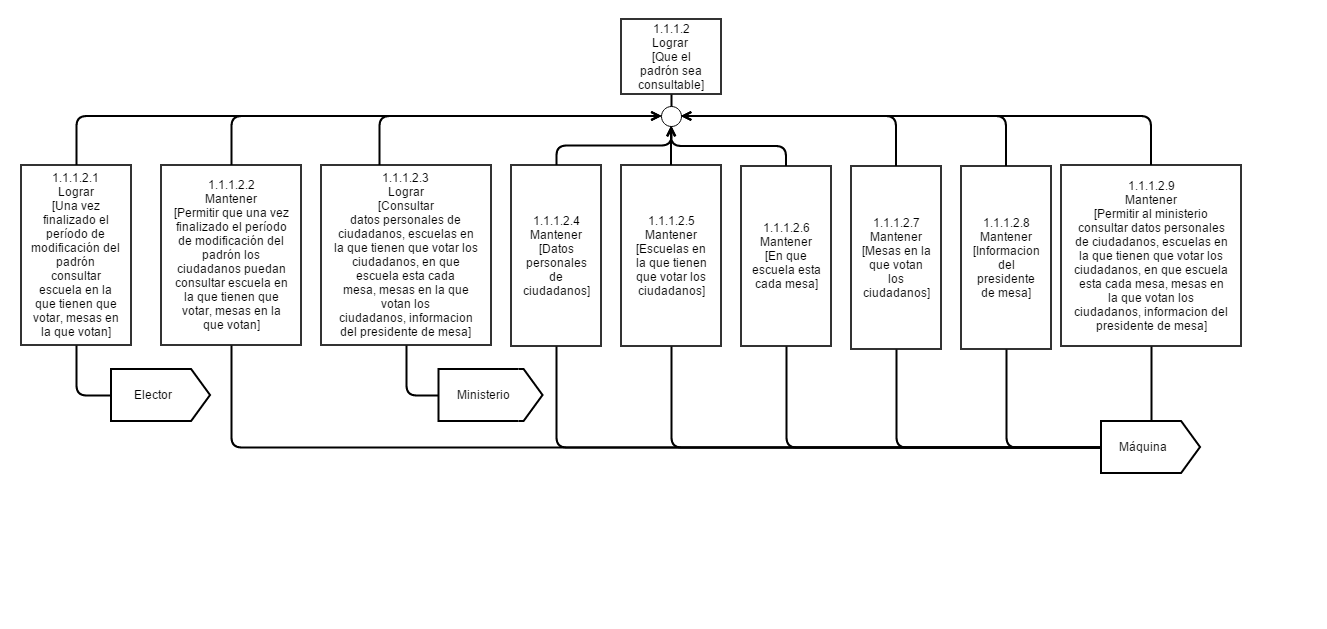
\includegraphics[scale=0.54]{imagenes/Diagramas/11/1112.png}
\\
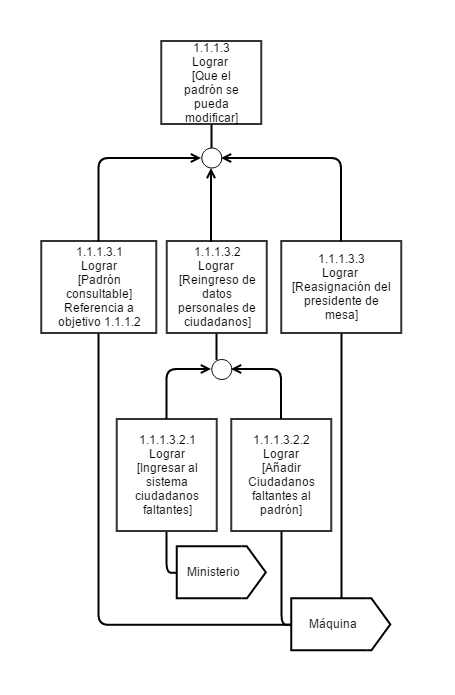
\includegraphics[scale=0.55]{imagenes/Diagramas/11/1113.png}
\\
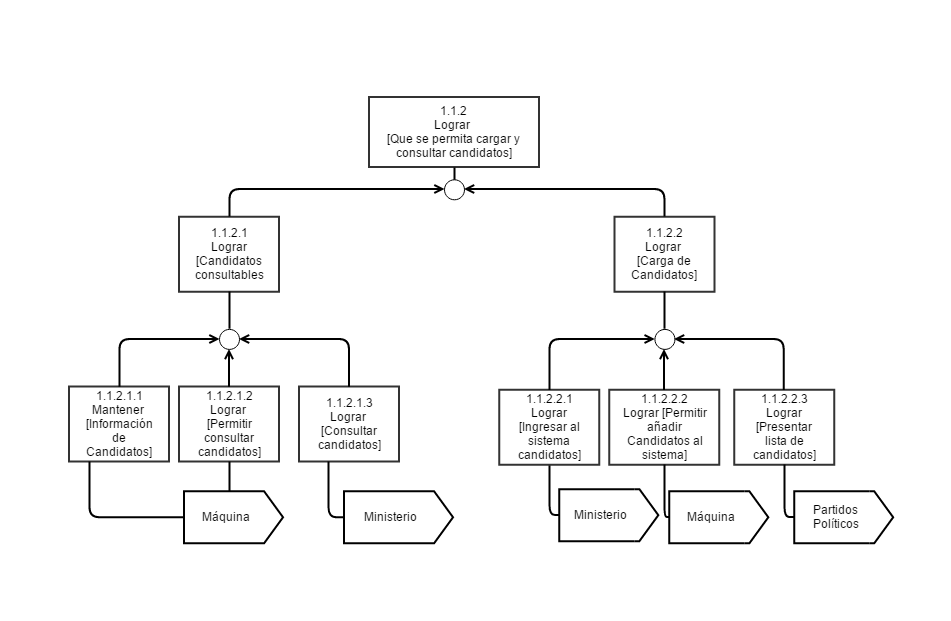
\includegraphics[scale=0.55]{imagenes/Diagramas/11/112.png}
\\
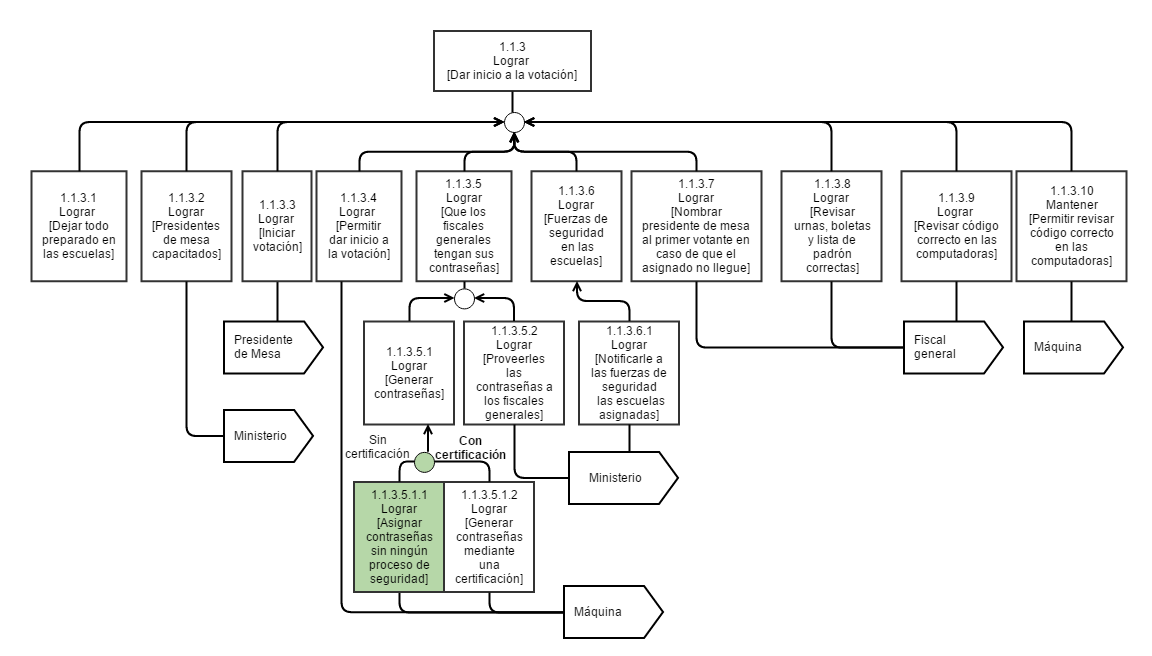
\includegraphics[scale=0.55]{imagenes/Diagramas/11/113.png}
\\
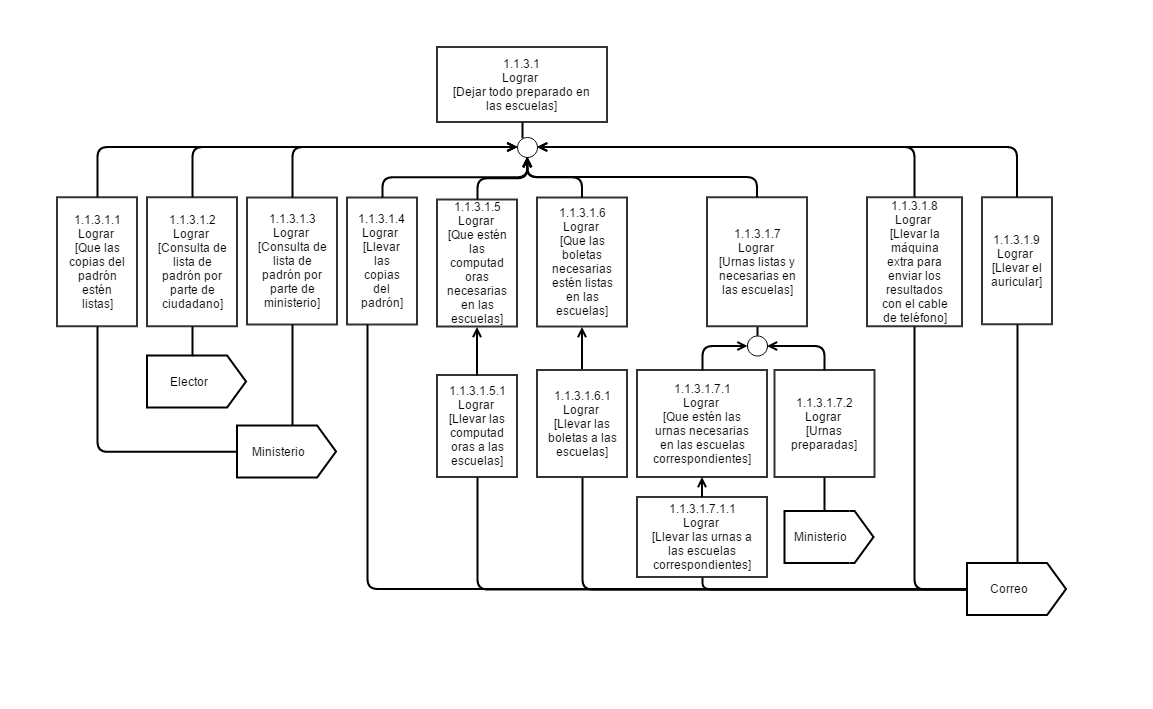
\includegraphics[scale=0.55]{imagenes/Diagramas/11/1131a.png}
\\
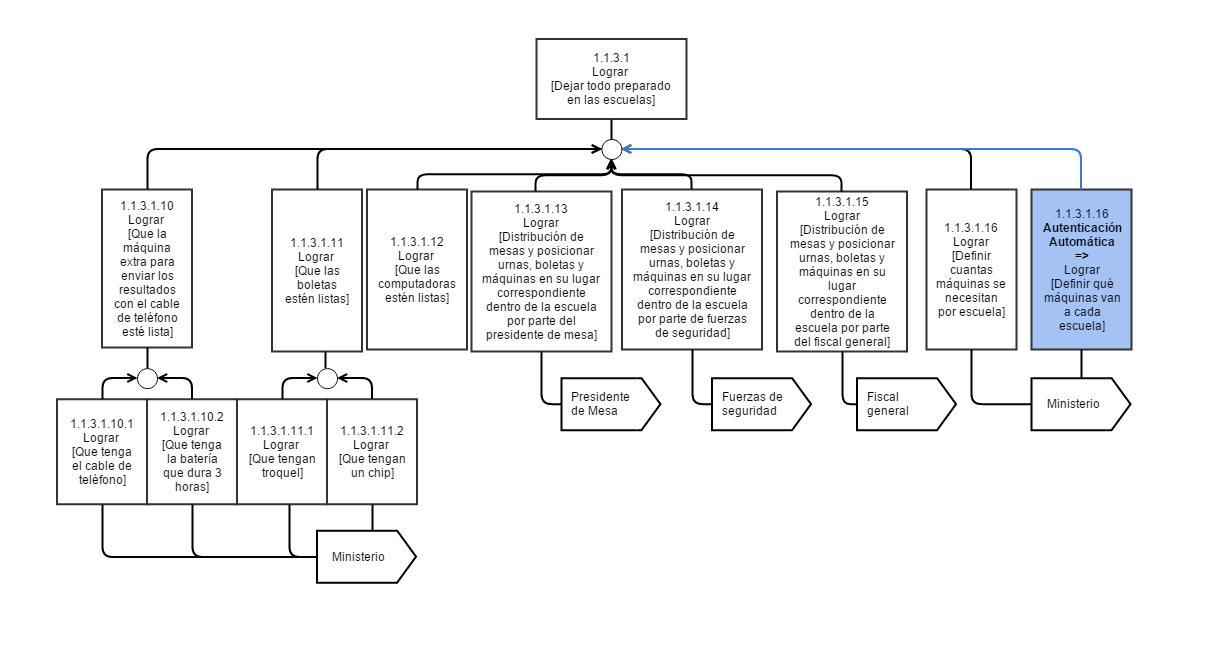
\includegraphics[scale=0.55]{imagenes/Diagramas/11/1131b.png}
\\
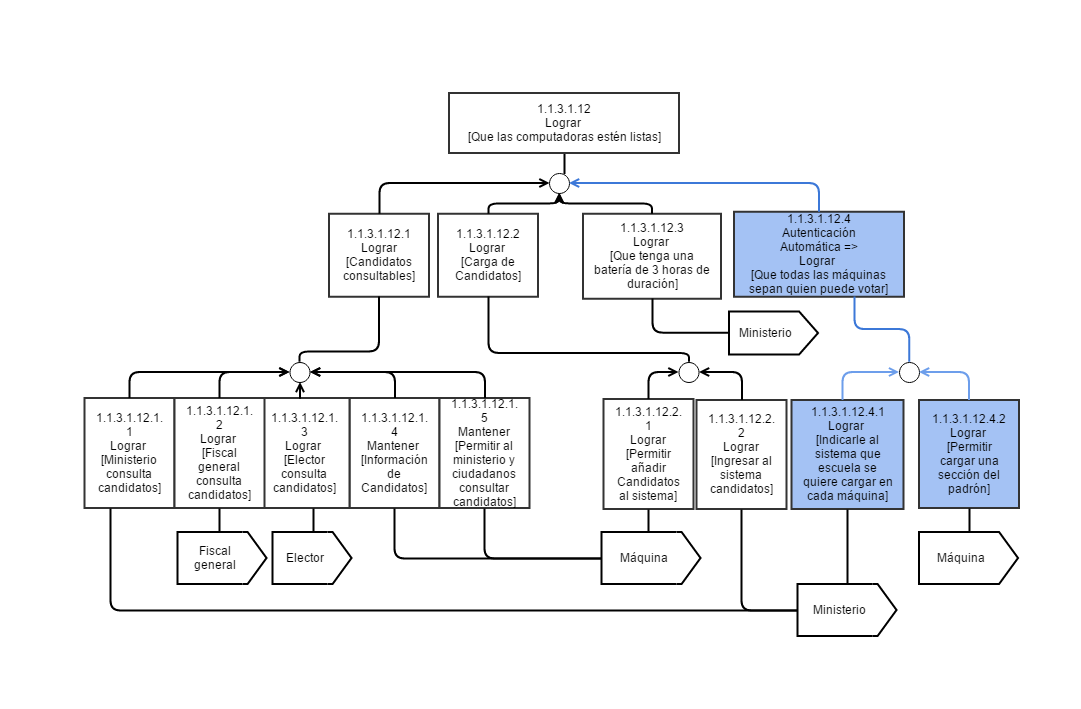
\includegraphics[scale=0.55]{imagenes/Diagramas/11/113112.png}
\\
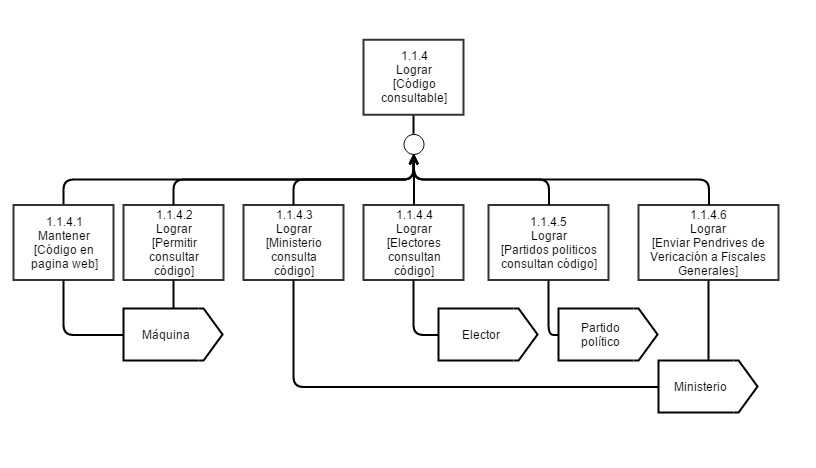
\includegraphics[scale=0.55]{imagenes/Diagramas/11/114.png}




\newpage
\subsection{Lista de requerimientos}

Dado el diagrama de objetivos, podemos rescatar de él un conjunto de requerimientos para 
nuestro sistema. Especificamente todos los objetivos que tengan como agente a la 
\textit{máquina} serán parte del listado de requerimientos de nuestro software.\\


Presentamos a continuación los requerimientos que se decantan de esta sección del diagrama de 
objetivos:

\begin{itemize}
\item Permitir asignación automatica de escuela y mesa a los ciudadanos
\item Permitir asignación de presidente de mesa
\item Permitir la carga de datos personales de ciudadanos
\item Permitir carga de escuelas disponibles
\item Asignar aleatoriamente presidente de mesa
\item Permitir que una vez finalizado el período de modificación del padrón los ciudadanos puedan consultar escuela en la que tienen que votar, mesas en la que votan
\item Permitir al ministerio consultar datos personales de ciudadanos, escuelas en la que tienen que votar los ciudadanos, en que escuela esta cada mesa, mesas en la que votan los ciudadanos, informacion del presidente de mesa
\item Permitir padrón consultable
\item Permitir añadir ciudadanos faltantes al padrón
\item Permitir reasignar presidente de mesa
\item Permitir consultar cantidatos
\item Permitir añadir candidatos al sistema
\item Generar contraseñas para fiscales generales 
\item Permitir revisar código
\item Mostrar código en web
\item Permitir código consultable
\item Permitir revisar código correcto en las computadoras

\end{itemize}

\newpage
\section{Diagrama de Objetivos (1.2)}

\subsection{Descripci\'on: Sufragio}


Llega un votante a la mesa. En caso de tener alguna discapacidad, tiene prioridad en la cola. 

Si el votante lo necesitase, podrá requerir ayuda y/o auriculares al presidente de mesa quien se deberá contactar con el Fiscal General con el fin de conseguir los auriculares. Para personas que posean problemas de movilidad, se les permitirá imprimir su voto en máquinas ubicadas en planta baja, mientras que el presidente de mesa les acercará la urna, para que pueda depositar su boleta al finalizar el sufragio. Sólo usará la máquina impresora de voto de la misma, mientras que es responsabilidad del presidente de mesa acercar la urna para que su voto sea contabilizado en la mesa que le corresponde por el padrón.

En el caso de que no posea una discapacidad, espera en la cola de votación de la mesa. 
En ambos casos, cuando es su turno, el votante le entrega su DNI al presidente de mesa. Este verifica su identidad al asegurarse que la persona que le entregó el DNI es la poseedora del mismo, que se encuentra en el padrón correspondiente a la mesa, y que no votó todavía. Los fiscales de mesa hacen lo mismo. Si hay algún problema, el presidente de mesa y/o los fiscales notifican al fiscal general de la escuela. El mismo decidirá si la persona está apta para emitir voto o no.\\

Si el votante pasa la verificación, el presidente de mesa procede a entregarle la boleta y le retiene el DNI. A la boleta entregada, le quita un troquel que posee el código identificatorio, dejándola con el otro código idéntico en la boleta.
Luego, el votante se acerca la máquina impresora de voto e inserta la boleta.\\

Entonces, el sistema de la máquina muestra por pantalla las opciones de votar por categoría o votar lista completa. Para ambos casos, se presentan las opciones (se incluye también la de voto en blanco) en posiciones aleatorias en la pantalla.

El votante podrá entonces elegir entre las opciones y al finalizar, obtener la boleta con su voto impreso (tanto en el papel como en el chip). El votante puede verificar en la máquina que lo impreso en el chip sea correcto.\\

Luego, el votante quita el troquel restante a la boleta, se lo entrega al presidente de mesa y si coincide con el retirado previamente, puede pasar a depositar la boleta en la urna siempre y cuando no haya cantado cuál será su voto. Si el votante canta su voto, la boleta quedará anulada impidiéndole ingresarla en la urna. 

Si el votante se arrepiente, puede pedir otra boleta y repetir el proceso.
Finalmente, el presidente de mesa le hace firmar al votante el padrón, y le devuelve el DNI conjunto a la constancia de voto.\\

En el caso de que falle alguna máquina, se pueden reemplazar por las dos de repuesto que posee cada escuela las cuales estarán a cargo del fiscal general. Si en una escuela dejan de funcionar más de dos máquinas, se podrá compartir la maquina de sufragio entre mesas, pero cada boleta deberá ser depositada en la urna correspondiente.\\
\textcolor{red}{El fiscal general puede, en todo momento, utilizar el pendrive suministrado por el Ministerio, para chequear que el código que se ejecuta en cada máquina, es el correcto.}

Pasadas las 18hs, las fuerzas de seguridad cierran las puertas de las escuelas. Y una vez terminados los comicios, empieza el conteo.

\newpage
\subsection{Diagrama}

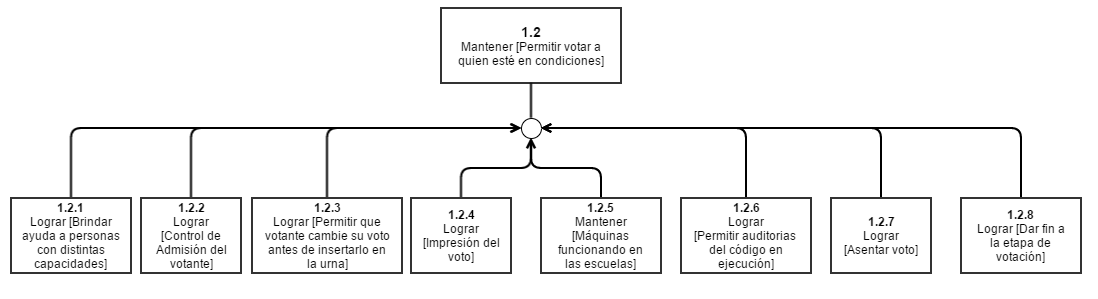
\includegraphics[scale=0.45]{imagenes/Diagramas/12/12.png}
\\
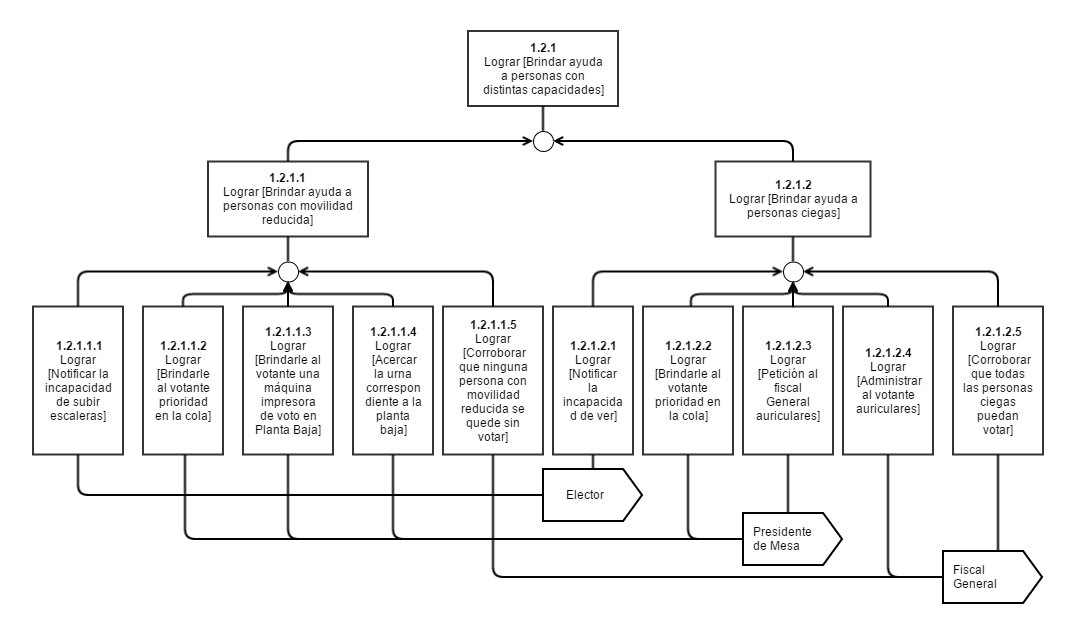
\includegraphics[scale=0.55]{imagenes/Diagramas/12/121.png}
\\
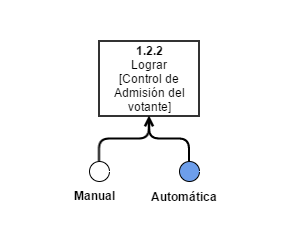
\includegraphics[scale=0.55]{imagenes/Diagramas/12/122.png}
\\
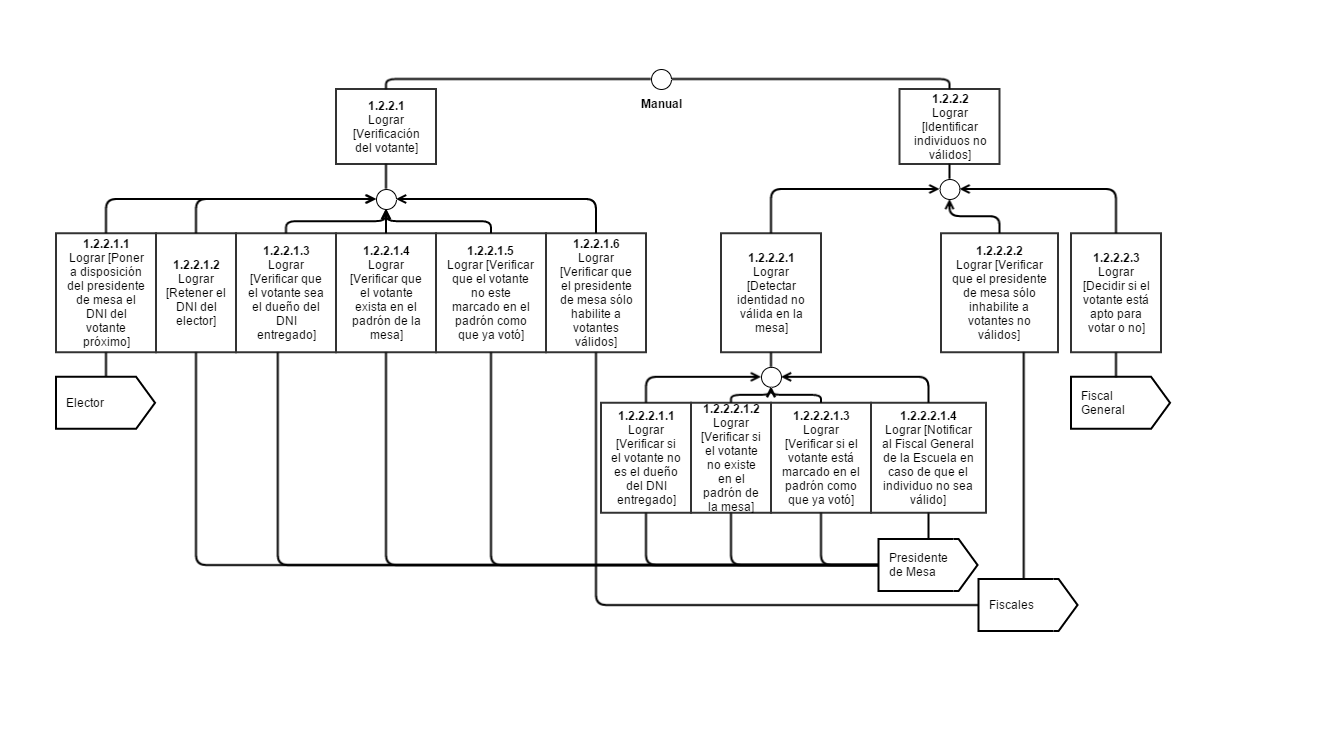
\includegraphics[scale=0.55]{imagenes/Diagramas/12/122a.png}
\\
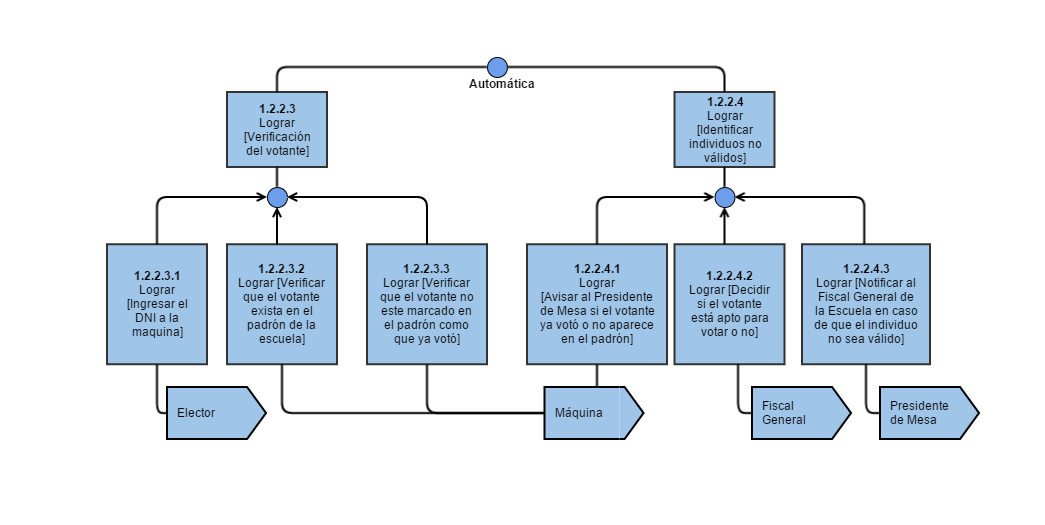
\includegraphics[scale=0.55]{imagenes/Diagramas/12/122b.png}
\\
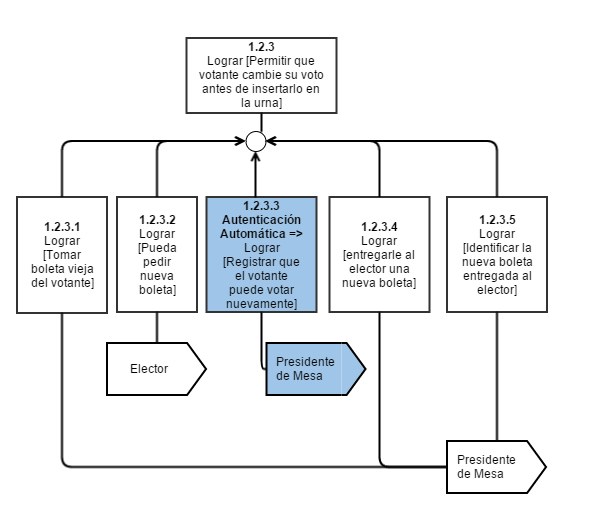
\includegraphics[scale=0.55]{imagenes/Diagramas/12/123.png}
\\
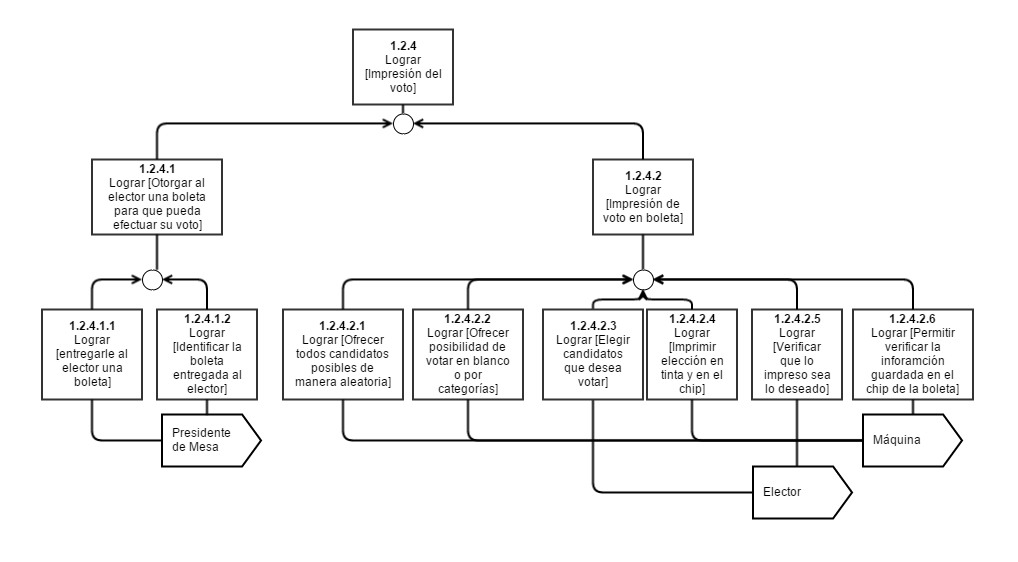
\includegraphics[scale=0.55]{imagenes/Diagramas/12/124.png}
\\
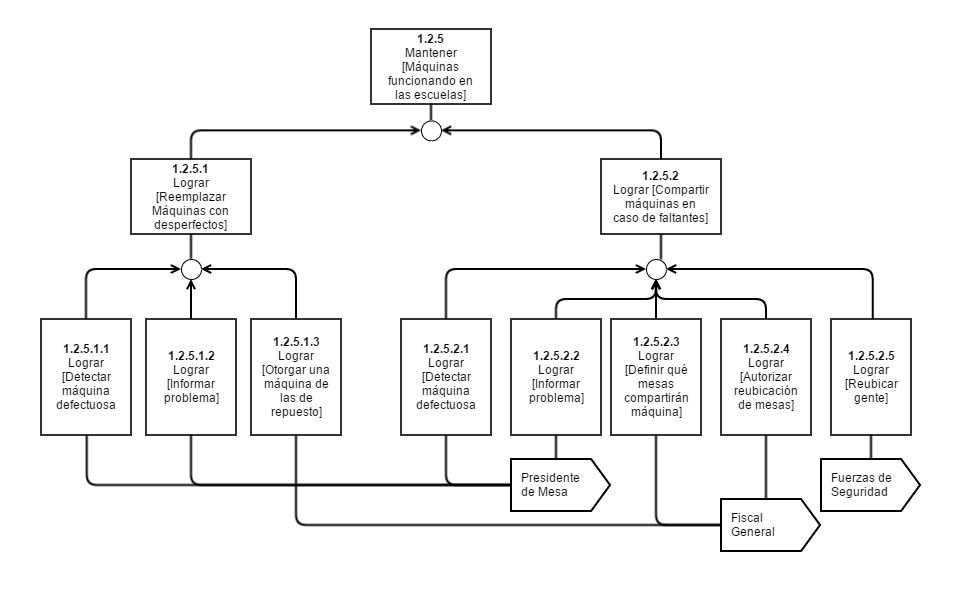
\includegraphics[scale=0.55]{imagenes/Diagramas/12/125.png}
\\
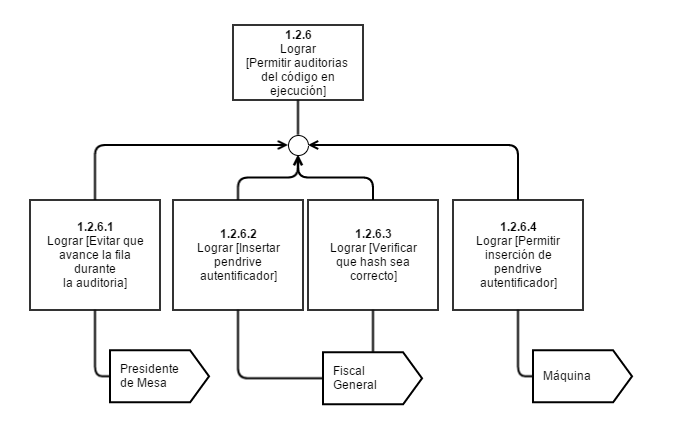
\includegraphics[scale=0.55]{imagenes/Diagramas/12/126.png}
\\
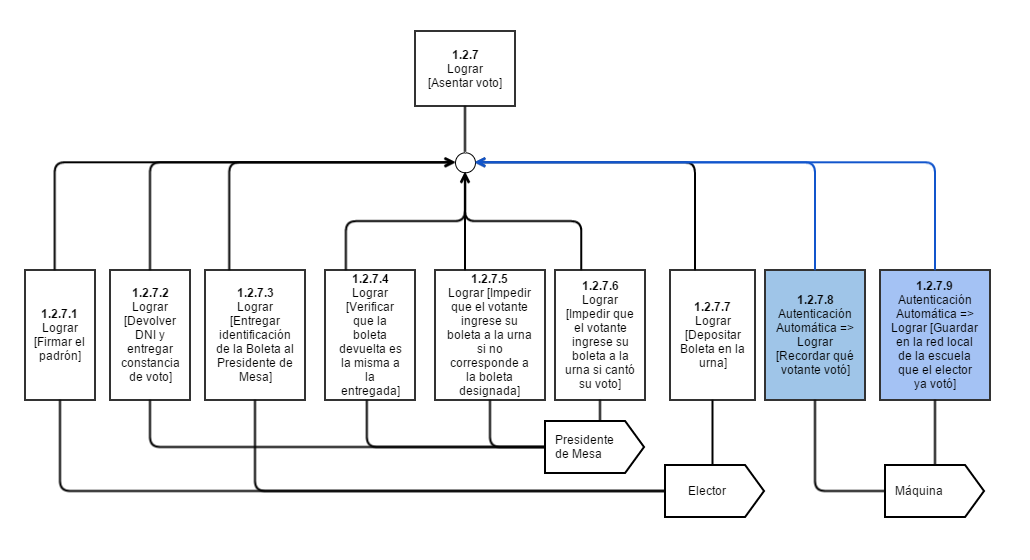
\includegraphics[scale=0.55]{imagenes/Diagramas/12/127.png}
\\
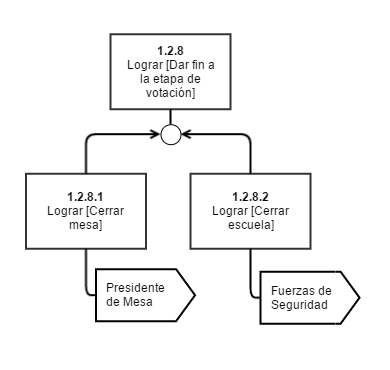
\includegraphics[scale=0.55]{imagenes/Diagramas/12/128.png}


\newpage
\subsection{Lista de requerimientos}

\begin{itemize}
\item Ofrecer todos los candidatos posibles de manera aleatoria
\item Ofrecer votar en blanco o en categorias
\item Imprimir elecciones en el chip y en tinta
\item Permitir la verificación de la información guardada en el chip
\item Permitir inserción de pendrive autentificador
\end{itemize}
\newpage
\section{Diagrama de Objetivos (1.3)}

\subsection{Descripci\'on: Conteo}


El presidente de mesa abre la urna y pone a la máquina impresora de voto en “Modo de conteo”, dando así comienzo al conteo de cada voto. En caso de que no haya nada impreso, o haya algo escrito a mano, se impugna el voto.

Cuando la máquina lee el chip, lleva la cuenta de los votos procesados. Al pasar la boleta por la máquina, figura en la pantalla el voto grabado. Se verifica que lo leído por el lector del chip, coincida con lo impreso en el papel. Los fiscales observan con detenimiento.\\

En caso de que ocurra alguna irregularidad, el presidente de mesa y/o fiscales lo comunicarán al fiscal general de la escuela. Frente a esta irregularidad, el fiscal general podrá anular la mesa (si lo considera necesario), por lo que no se enviaría el resultado al centro de Cómputos.\\

Al finalizar el conteo, el presidente de mesa insertará una boleta vacía en la máquina impresora de voto, la cual grabará en el chip los resultados contabilizados de la mesa. Además imprimirá con tinta en la boleta los ganadores de cada categoría para así obtener una manera de contrastar lo grabado con lo contabilizado.
Luego, el presidente de mesa llevará la boleta con el conteo al Fiscal general, quien será el encargado de cargarla en la máquina de impresión de votos con conexión telefónica destinada al envío de resultados. El mismo posee dos contraseñas; al ingresar la primera, la máquina impresora de votos le permitirá ingresar al “Modo envío”. Una vez cargadas todas las boletas, las envía por el enlace telefónico al centro de cómputos nacional, enviándole también su contraseña única de Fiscal General. El presidente de mesa podrá acompañarlo en todo momento para ver que se contabilice lo correcto.\\
\textcolor{red}{El fiscal general puede, en todo momento, utilizar el pendrive suministrado por el Ministerio, para chequear que el código que se ejecuta en cada máquina, es el correcto.}\\
Posteriormente, el presidente de mesa inserta la boleta con el conteo impreso en la urna junto a todas las boletas contabilizadas de la mesa. El presidente sella la urna, el fiscal general la agrupa con las otras que hay en escuela, y brinda al correo todas las urnas de su escuela e identifica a las urnas que hayan sido impugnadas. Además, envía el padrón para poder identificar a quienes votaron. El correo se encarga de enviarlas al centro de cómputos nacional.\\

El Sistema del Centro de Cómputos sólo contabilizará resultados de mesas que hayan sido cargados con contraseñas de Fiscal General válidas y correspondientes a las mesas de las urnas recibidas.
El Centro de Cómputos nacional calcula los resultados provisorios de las elecciones (como si hay ballotage, o la cantidad de diputados mediante el método D’Hont) con la información recibida por el enlace telefónico.

A las 20hs el Centro de Cómputos nacional publica los resultados del conteo provisorio en su página web.\\

Finalmente, el correo llevará todas las urnas al centro de cómputos nacional donde se realizará el conteo definitivo (No es posible saber a priori cuándo ocurrirá esto).

\newpage
\subsection{Diagrama}

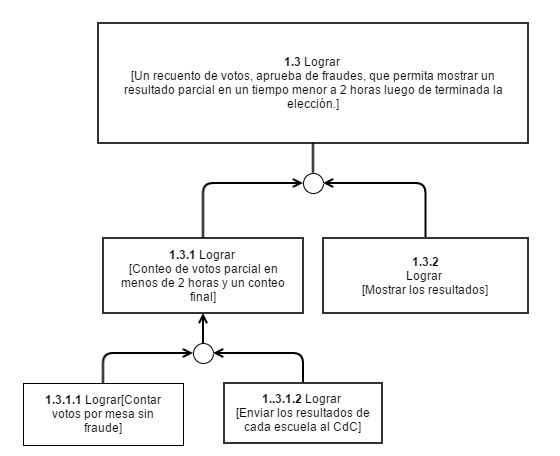
\includegraphics[scale=0.55]{imagenes/Diagramas/13/13.png}
\\
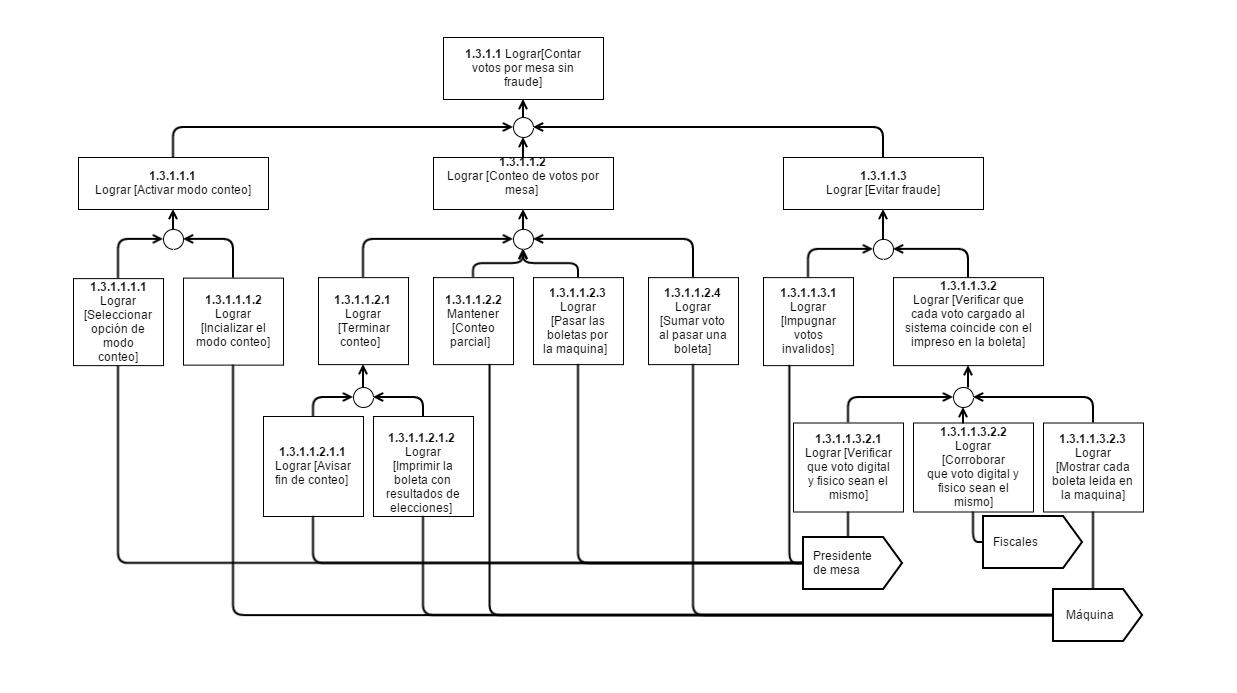
\includegraphics[scale=0.55]{imagenes/Diagramas/13/1311.png}
\\
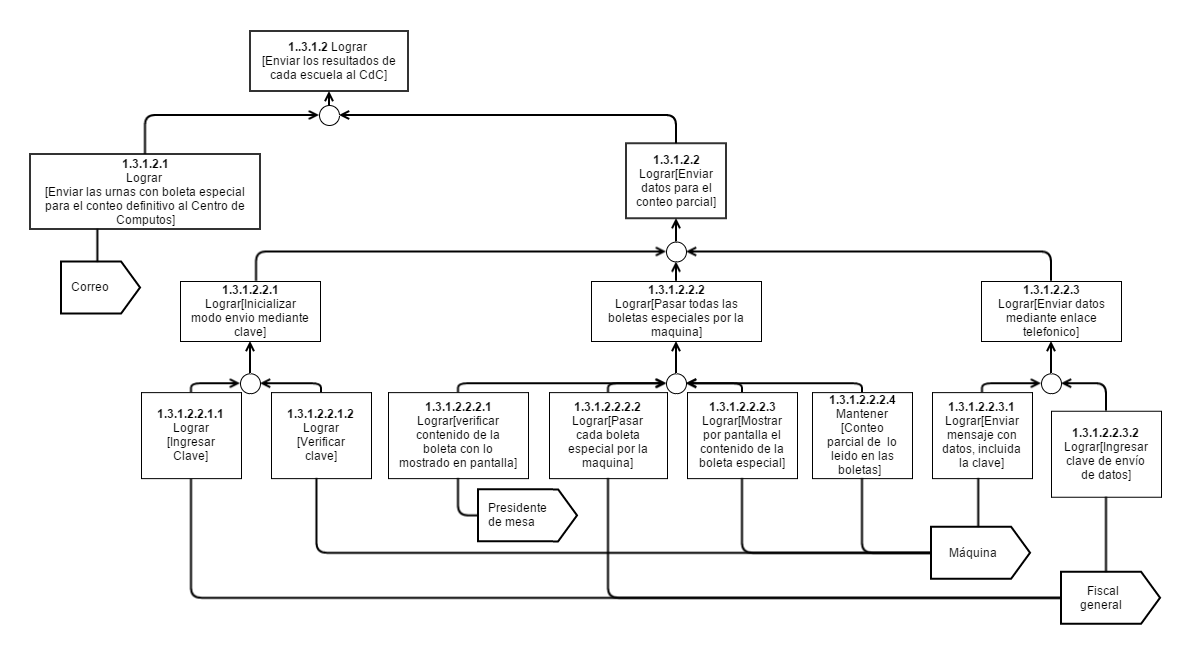
\includegraphics[scale=0.55]{imagenes/Diagramas/13/1312.png}
\\
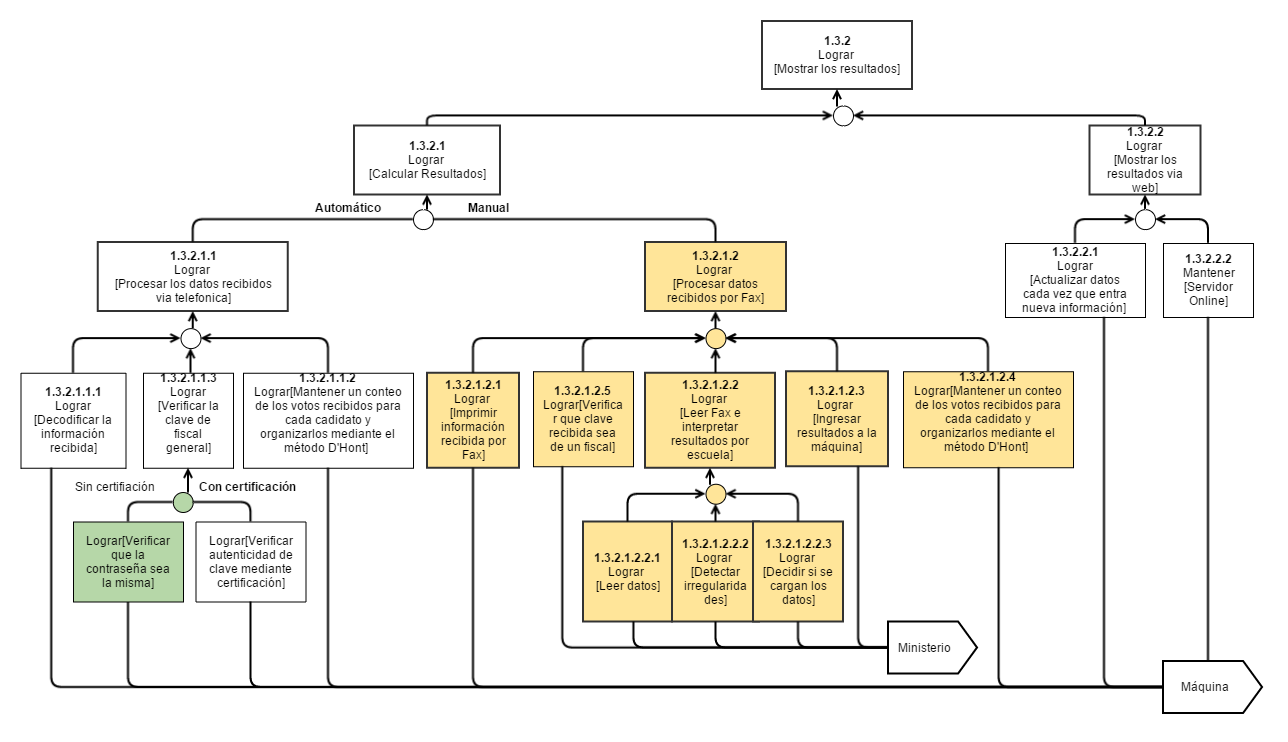
\includegraphics[scale=0.53]{imagenes/Diagramas/13/132.png}

\newpage
\subsection{Requerimientos de la m\'aquina}

Dada esta sección podemos obtener los siguientes requerimientos para nuestra maquina:
\begin{itemize}
\item Incializar Modo conteo
\item Sumar votos al pasar una boleta en modo conteo
\item Mantener un conteo parcial en modo conteo
\item Mostrar cada boleta leida en pantalla
\item Imprimir boleta especial para envio
\item Verificar clave para entrar en modo envio
\item Mantener un conteo parcial en el modo envio
\item Mostrar el contenido de la boleta especial
\item Enviar mensaje con los datos para el conteo parcial con la clave del fiscal general encriptada
\item Decodificar la información del mensaje
\item Mantener un conteo parcial de los datos recibidos para cada candidato y organizarlo según el método d'Hont
\item Verificar la clave del fiscal
\item Actualizar los resultados cuando entran datos
\item Mantenerse online
\end{itemize}
\newpage
\section{O-refinamientos}

En los diagramas presentados anteriormente se pueden ver distintos o-refinamientos (marcados cada uno con distintos colores de manera de poder ser distinguidos). A continuación haremos enfásis en cada uno de ellos compar\'andolos con la idea central presentada en el diagrama de objetivos. Para lograr una comparación interesante, utilizaremos tres criterios (es decir, objetivos blandos): transparencia, costo y rapidez.

\subsection{O-refinamiento 1: Claves de env\'io sin encriptación}

Este O-refinamiento es muy simple, no utiliza un sistema de certificados para el env\'io de los resultados del conteo de cada escuela.

Si bien esto lo hace más rapido al no ser necesario desencriptar mensajes y más barato, al no necesitar conseguir certificaciones de seguridad, la transparencia es menor. Cualquier persona que intercepte el mensaje puede obtener la contraseña y por lo tanto cambiar los resultados del 
conteo parcial. Si bien esto no influye en el conteo final que se realiza luego, cambia los resultados parciales eliminando mucha transparencia.

Presentamos una tabla comparativa de las dos maneras de lograr el env\'io de claves en función de los objetivos blandos presentados anteriormente:

\begin{table}[H]
\centering
 \begin{tabular}{|c | c | c | c|} 
 \hline
 & Rapidez & Tranparencia & Costo \\
 \hline
 método sin certificación & ++ & -  & -- \\
 \hline
 método con certificación & - & ++ & + \\
 \hline
 
 \end{tabular}
\end{table}

\subsection{O-refinamiento 2: Auntentificación automática del votante}

La idea detrás de este O-refinamiento es asignar a la máquina la tarea de identificar al votante, dejando como única tarea para el presidente de mesa revisar y entregar boletas.

Entonces el proceso de votación cambiar\'ia, como está indicado en 1.2 del diagrama de objetivos bajo el tag \textbf{automático}.

La idea es la siguiente, existe una urna por maquina, pero cualquier persona puede votar en cualquier m\'aquina. Cuando una persona llega, elige una m\'aquina y se sitúa en la cola de la misma. Cuando es su turno, el presidente de mesa se queda con un troquel, y le da la boleta.

El votante va a la m\'aquina, pasa su dni, por una ranura especial y el sistema lo identifica como votante válido. Si la maquina no lo reconoce como votante válido o aparece que el votante ya votó, emite una señal sonora para que el presidente de mesa llame al fiscal general y analice la irregularidad. Si lo reconoce, el votante inserta la boleta y vota normalmente.

Una vez que votó, quita el segundo troquel, el presidente lo verifica, e inserta la boleta en la urna. Una vez que se imprimió el voto, la maquina se comunica mediante wifi con todas las otras máquinas de la escuela para avisar que esa persona ya votó. De manera de evitar que la misma persona vote más de una vez.

Si el votante se arrepiente de su voto después de imprimir la boleta, pero antes de insertarla en la urna, el presidente de mesa tiene que acceder a cualquiera de las máquinas y hacer que la persona en cuestión aparezca como que todavía no voto.

Los fiscales deben verificar que todo sea legal, para que el presidente de mesa no se aproveche de esta función y haga fraude.

Si bien este método es más r\'apido, tiende a tener mayores irregularidades, el presidente de mesa podría cambiar votos de manera muy simple. 

\begin{table}[H]
\centering
 \begin{tabular}{|c | c | c | c|} 
 \hline
 & Rapidez & Tranparencia & Costo \\
 \hline
 método clasico & + & ++  & -- \\
 \hline
 método automático & ++ & -- & ++ \\
 \hline
 
 \end{tabular}
\end{table}


\subsection{O-refinamiento 3: recibir datos por fax}

La idea de este o-refinamiento es que en vez de enviar una mensaje codificado por el enlace telefonico, utilizar el mismo para enviar un fax. De esta manera en alguna locación definida, personal del ministerio recibe el fax, verifica que no contenga irregularidades y lo carga en un sistema interno que lleva el conteo de los datos.

El gran problema de esto es la velocidad en que sucede, ya que al requerir que un humano verifique el contenido de cada fax esto lleva tiempo. Además subir los datos al sistema depende de un humano y esto puede implicar que cambie los resultados.

Comparemoslo entonces con el método automatizado de que la maquina procese directamente el mensaje enviado por el enlace telefonico.

\begin{table}[H]
\centering
 \begin{tabular}{|c | c | c | c|} 
 \hline
 & Rapidez & Tranparencia & Costo \\
 \hline
 método automático & ++ & ++  & ++ \\
 \hline
 método manual & -- & -- & -- \\
 \hline
 
 \end{tabular}
\end{table}
\newpage
\section{Diagrama de Contexto}

%\includegraphics[scale=0.55]{imagenes/contextocentrocomputo.png}

\newpage

%\includegraphics[scale=0.6]{imagenes/contextomaquinasufragio.png}

%\normalsize
%\newpage

%\section{Objetivos generales}

%El objetivo de este Trabajo Práctico es ...


%\section{Contexto}

%\begin{figure}
%  \begin{center}
%	
\includegraphics[scale=0.66]{imagenes/logouba.jpg}
%	\caption{Descripcion de la figura}
%	\label{nombreparareferenciar}
%  \end{center}
%\end{figure}


%\paragraph{\textbf{Titulo del parrafo} } Bla bla bla bla.
%Esto se muestra en la figura~\ref{nombreparareferenciar}.



%\begin{codesnippet}
%\begin{verbatim}

%struct Pepe {

%    ...

%};

%\end{verbatim}
%\end{codesnippet}


%\section{Enunciado y solucion} 
%\input{enunciado}

%\section{Conclusiones y trabajo futuro}


\end{document}

